% TU Delft beamer template
% Author: Erwin Walraven (initial version was created by Maarten Abbink)
% Delft Universiy of Technology

\documentclass{beamer}
\usepackage[english]{babel}
\usepackage{calc}
\usepackage[absolute,overlay]{textpos}
\usepackage{graphicx}
\usepackage{subfig}
\usepackage{amsmath}
\usepackage{amsfonts}
\usepackage{amsthm}
\usepackage{mathtools}
\usepackage{comment}
\usepackage{MnSymbol,wasysym}
\usepackage{url}
\usepackage{fancyhdr}
\usepackage{etoolbox}
\usepackage{graphicx}
\usepackage{float}
\usepackage{qcircuit}
\usepackage	{caption}
\usepackage{graphicx}




\setbeamertemplate{navigation symbols}{} % remove navigation symbols
%\mode<presentation>{\usetheme{tud}}
\usetheme{Hannover}
\addtobeamertemplate{navigation symbols}{}{%
	\usebeamerfont{footline}%
	\usebeamercolor[fg]{footline}%
	\hspace{1em}%
	\insertframenumber/\inserttotalframenumber
}

% BIB SETTINGS
\usepackage[backend=bibtex,firstinits=true,maxnames=30,maxcitenames=20,url=false,style=authoryear]{biblatex}
\bibliography{bibfile}
\setlength\bibitemsep{0.3cm} % space between entries in the reference list

% Commands
\renewcommand{\vec}[1]{\boldsymbol{#1}}
\renewcommand{\bibfont}{\normalfont\scriptsize}
\setbeamerfont{footnote}{size=\tiny}
\renewcommand{\cite}[1]{\footnote<.->[frame]{\fullcite{#1}}}
\newcommand{\gambe}{\vec{\gamma},\vec{\beta}}
\newcommand{\backupbegin}{\newcounter{finalframe}
	\setcounter{finalframe}{\value{framenumber}}}
\newcommand{\backupend}{\setcounter{framenumber}{\value{finalframe}}}
\def\vfilll{\vskip 0pt plus 1filll minus 0pt }
\newcommand\blfootnote[1]{%
	\begingroup
	\renewcommand\thefootnote{}\footnote{#1}%
	\addtocounter{footnote}{-1}%
	\endgroup
}

\title[]{Quantum Approximate Optimization Algorithm}
\subtitle{Performance on Max-Cut using Heuristic Parameter determination}
\institute[]{Delft University of Technology, the Netherlands}
\author{Joost Bus}
\date{23 July 2020}


\begin{document}
{\setbeamertemplate{footline}{\usebeamertemplate*{minimal footline}}
\begin{frame}
\vfilll
\titlepage
\footnotesize
\centering
\begin{tabular}{c}
	\textbf{Supervisors} \\
	Matthias M\"{o}ller \\
	Carmina G. Almudever
\end{tabular}%
\vfilll
\tiny{Contact: \url{j.c.p.bus@student.tudelft.nl}}
\end{frame}
{\setbeamertemplate{footline}{\usebeamertemplate*{minimal footline}}}

% Overview
\begin{frame}{Overview}
\tableofcontents
\end{frame}

\section{Quantum computing}
\begin{frame}{Why Quantum Computing?}

\begin{columns}
	\begin{column}{.49\textwidth}
		\begin{itemize}
			\item Medicine
			\item Chemistry
			\item Cryptography
			\item Optimization
		\end{itemize}
	\end{column}
	\begin{column}{.49\textwidth}
		\begin{figure}
			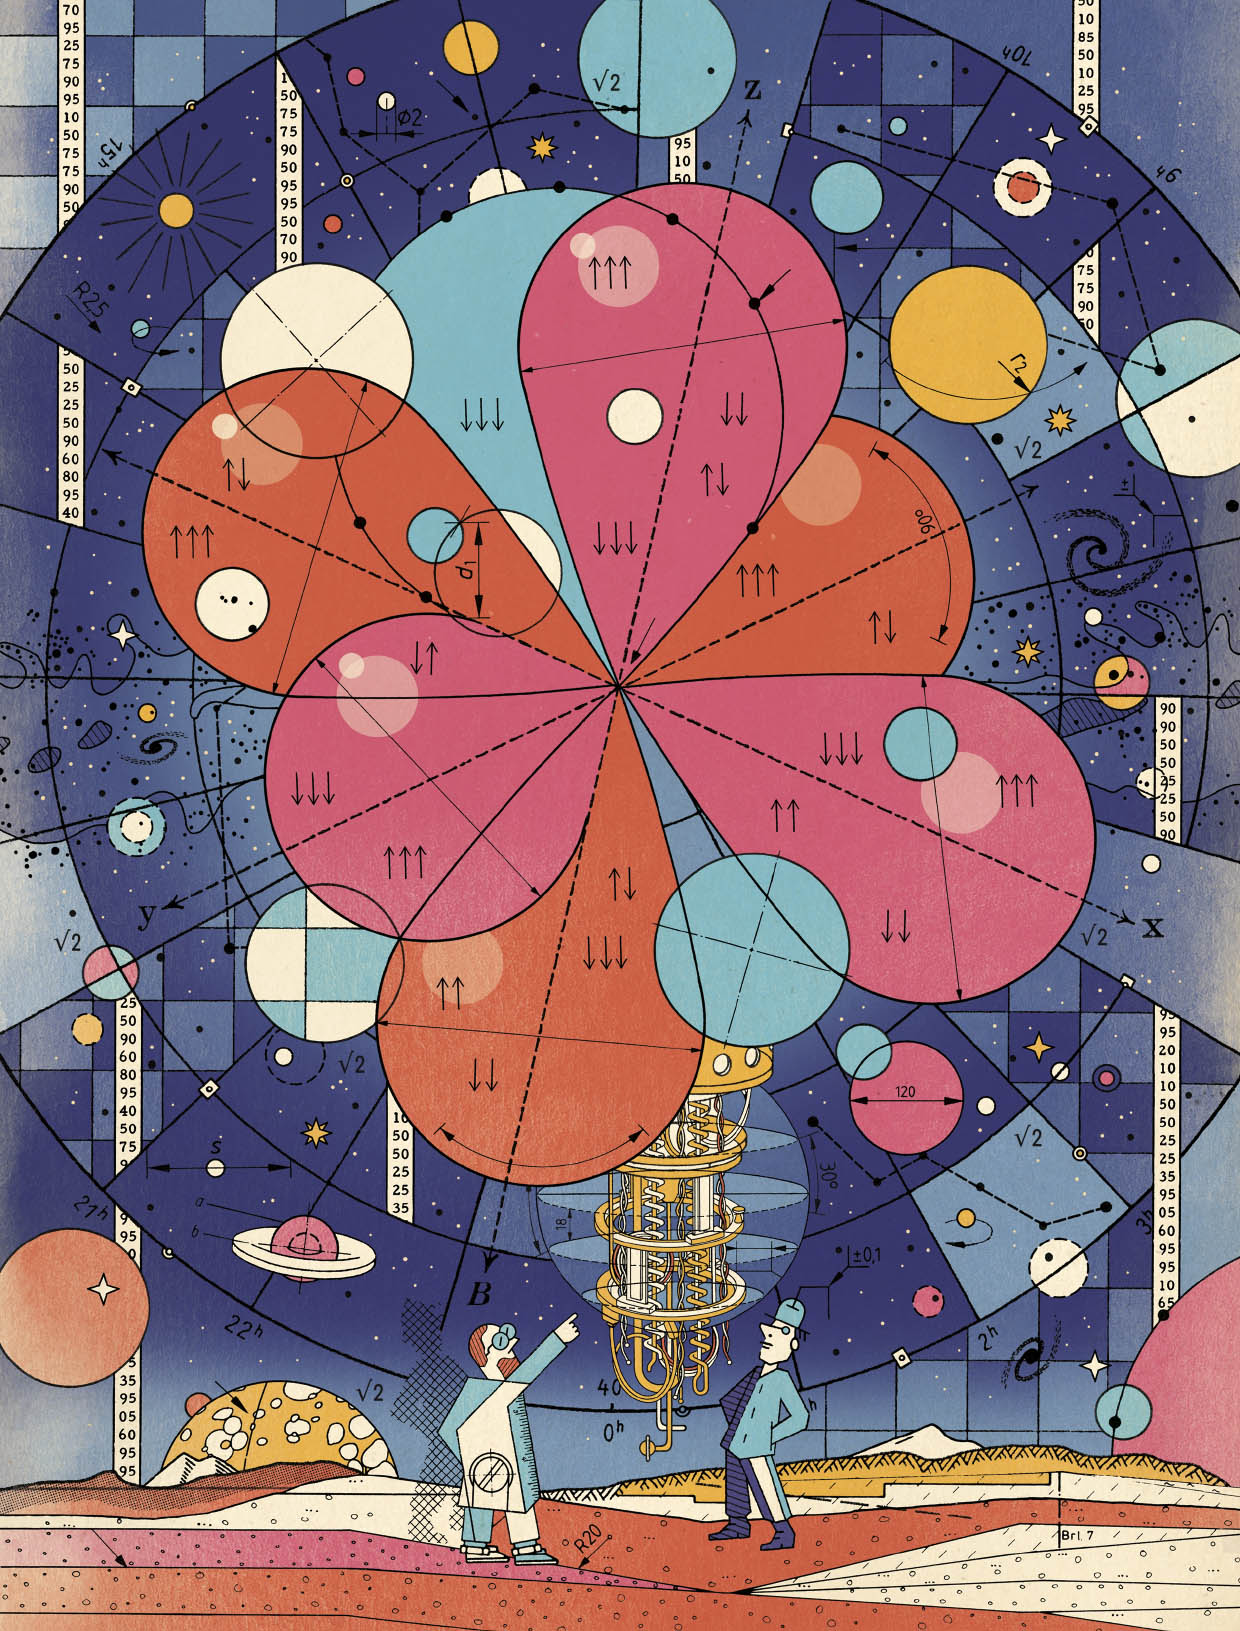
\includegraphics[width=\textwidth]{figures/cartoon}
		\end{figure}
		
	\end{column}
\end{columns}
\blfootnote{Illustration by Christian Gralingen}
\end{frame}

\begin{frame}{Are we there yet?}
The current state of Quantum Computers
\begin{itemize}
	\item $10 \: {\raise.17ex\hbox{$\scriptstyle\sim$}} \: 100$ qubits
	\item Limited connectivity
	\item Non-negligible error rates
	\item No error correction
\end{itemize}
\vspace{20px}
\pause
\textbf{Do current devices still have useful applications?}
\end{frame}

\begin{frame}{Are we there yet?}
\textbf{Do current devices still have useful applications?}
\begin{figure}
	\centering
	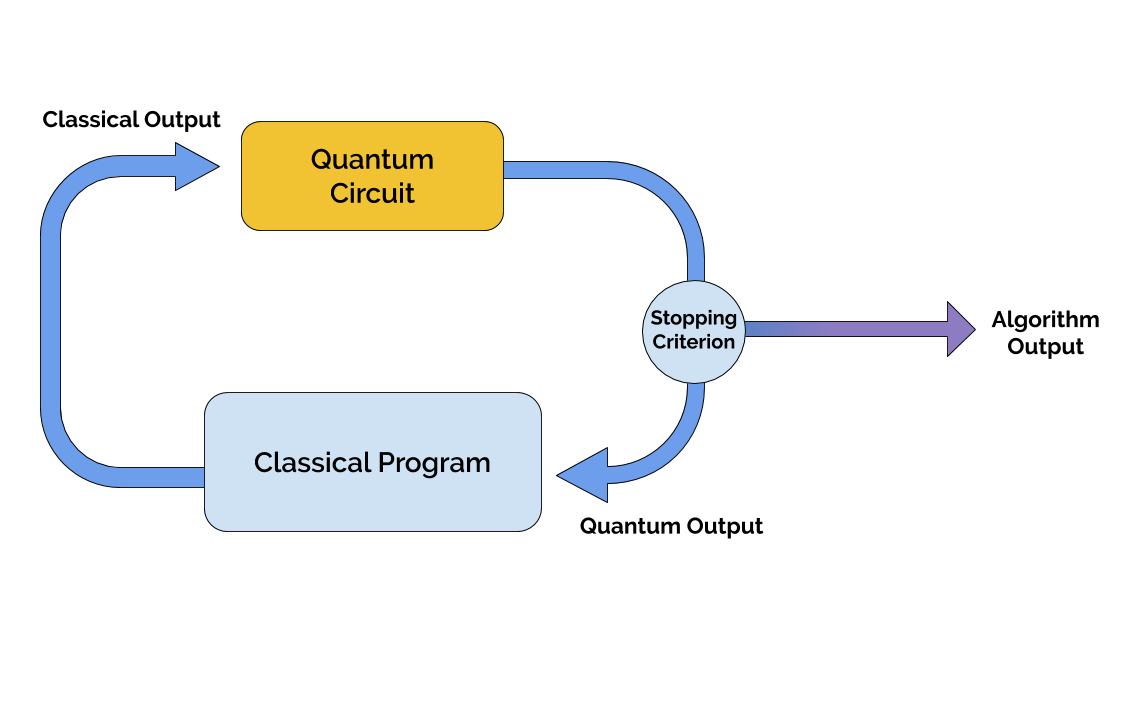
\includegraphics[width=0.9\textwidth]{figures/hybrid}
\end{figure}
\blfootnote{Figure from Entropica Labs}
\end{frame}

%\begin{frame}{Are we there yet?}
%It is possible to run hybrid algorithms with short quantum circuits
%\begin{figure}
%	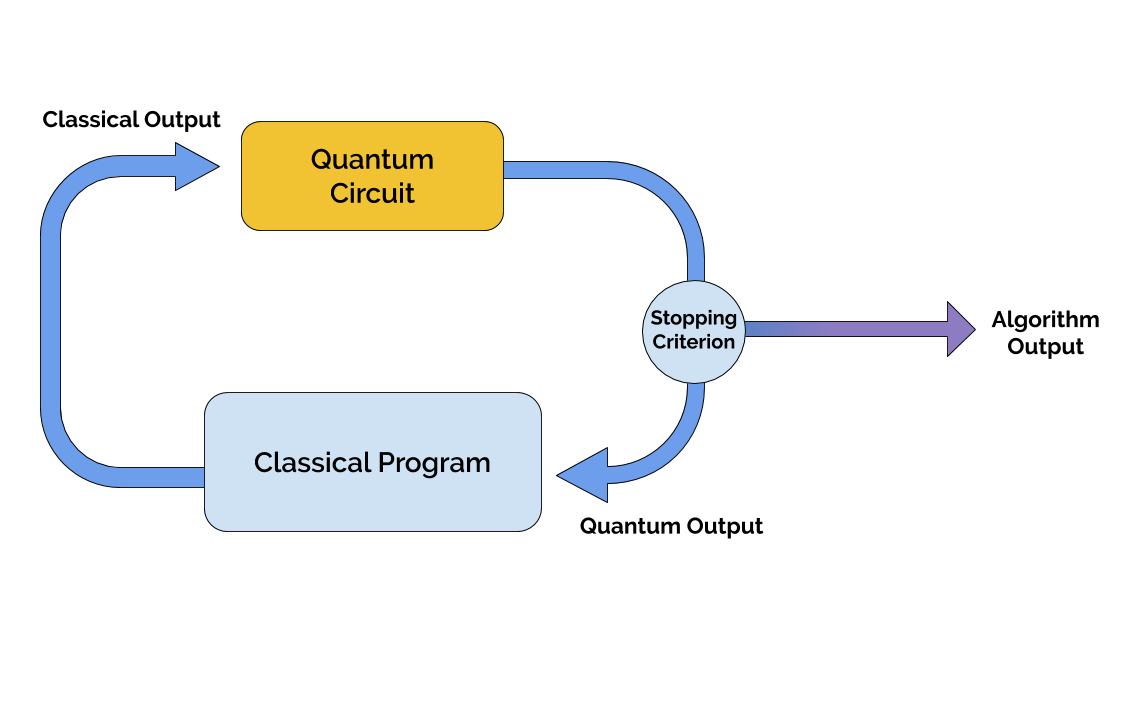
\includegraphics[width=0.8\textwidth]{figures/hybrid}
%\end{figure}
%\blfootnote{Figure from Entropica Labs}
%\end{frame}

\begin{frame}{Quantum Computing - The basics}
\begin{figure}
	\centering
	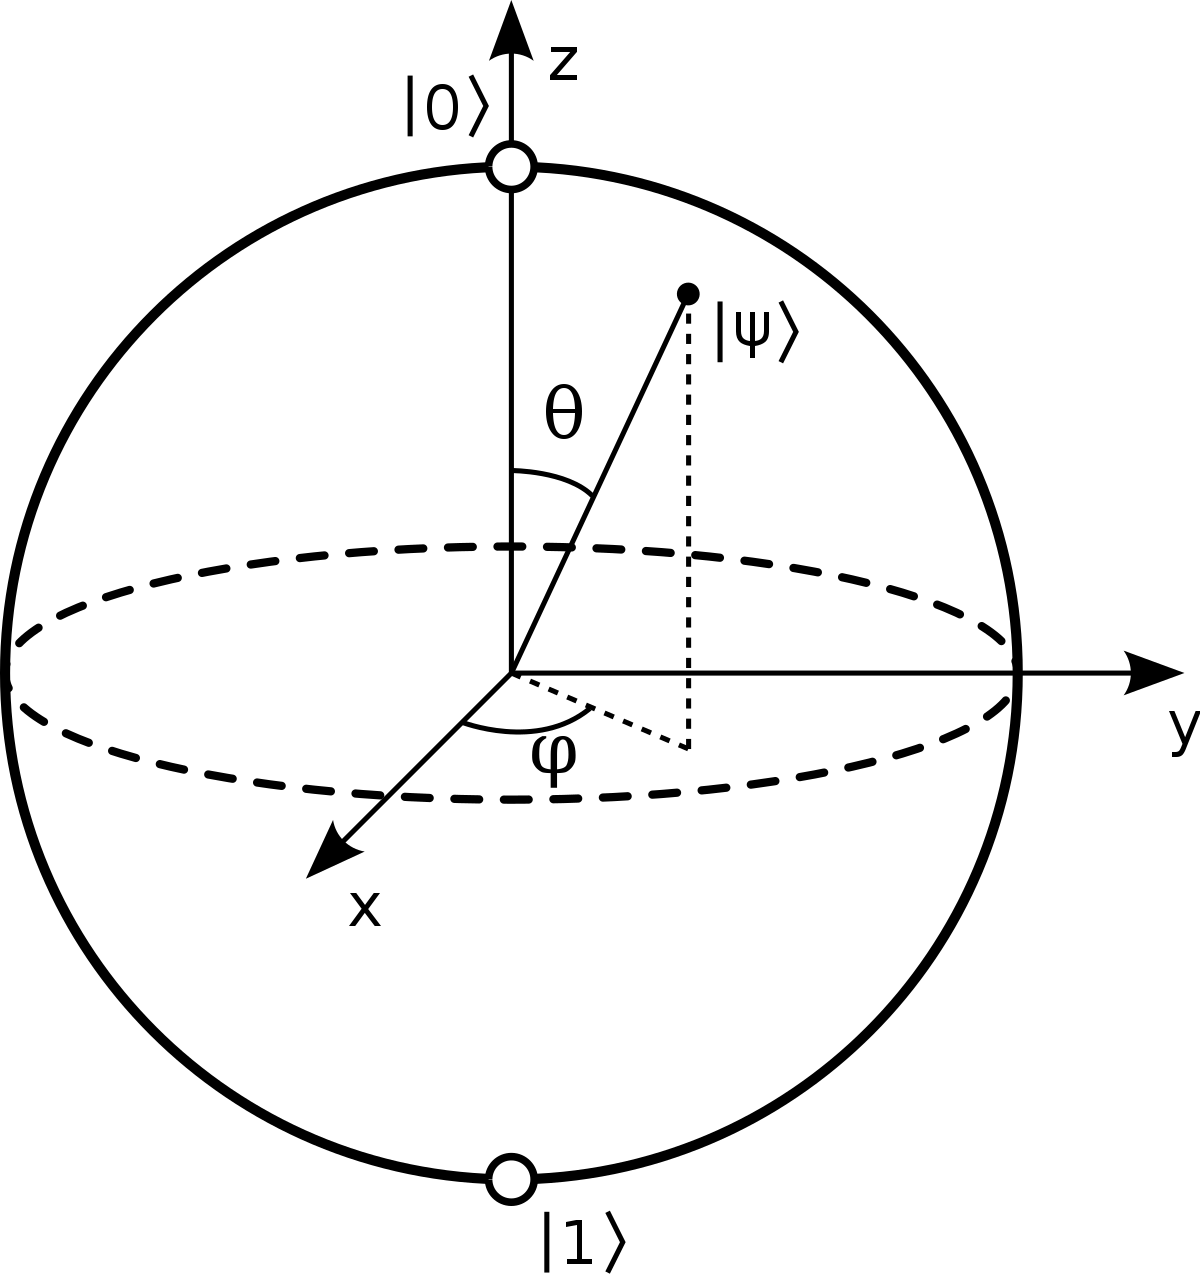
\includegraphics[width=0.4\textwidth]{figures/Bloch.png}
\end{figure}
\blfootnote{Figure from Wikipedia - Bloch sphere}
\end{frame}

\begin{frame}{Quantum Computing - The basics}
One quantum bit or qubit can be described as a \textbf{superposition}, or (linear) combination of two states with corresponding \textbf{amplitudes}
\begin{equation}
	|\psi\rangle = \alpha_1|0\rangle + \alpha_2|1\rangle 
\end{equation}
\pause
Similarly, for a two qubit system we the system is described with four amplitudes.
\begin{equation}
	\alpha_1|00\rangle + \alpha_2|01\rangle + \alpha_3|10\rangle + \alpha_4|11\rangle
\end{equation}
\pause
In general, we need $2^n$ amplitudes to describe an $n$ qubit system and some say the system is in $\mathbf{2^n}$ \textbf{states} ``at the same time''. Hence the exponential power of the quantum computer.
\begin{equation}
	\alpha_1|0\dots 0\rangle + \dots + \alpha_{2^n}|1\dots 1\rangle
\end{equation}
\end{frame}

\begin{frame}{Quantum Computing - The basics}
	\textbf{However}, we are not able to measure the amplitudes directly. Upon measurement, the system \textbf{collapses} into \emph{one} classical state with  probability related to the magnitude of the corresponding amplitude. 
\end{frame}

\begin{frame}{Quantum Computing - The basics}
\textbf{Example with 2 qubits}\\~\\
	Given the following system
	
	\begin{equation}
	\alpha_1|00\rangle + \alpha_2|01\rangle + \alpha_3|10\rangle + \alpha_4|11\rangle
	\end{equation}
	
	we find the following results with their corresponding probabilities
	\begin{table}
		\centering
		\begin{tabular}{||c c c||} 
			\hline
			State & Amplitude & Probability \\ [0.5ex] 
			\hline\hline
			00 & $\alpha_1$ & $|\alpha_1|^2$ \\ 
			01 & $\alpha_2$ & $|\alpha_2|^2$ \\
			10 & $\alpha_3$ & $|\alpha_3|^2$ \\
			11 & $\alpha_4$ & $|\alpha_4|^2$ \\ [1ex] 
			\hline
		\end{tabular}
	\end{table}
\end{frame}

\begin{frame}{Quantum Computing - The basics}
	So the amplitudes have a special meaning: \textbf{the squared magnitude signifies the probability of a particular state.} We can change the amplitudes by applying \textbf{gates}, which are descibed by (unitary) matrices.\\~\\
	
	%\pause
	%The art of quantum computing is to choose a sequence of gates in such a way that desirable states are amplified, and bad states are suppressed.
	\pause
	\begin{columns}
		\begin{column}{0.4\textwidth}  %%<--- here
			\begin{figure}[b]
				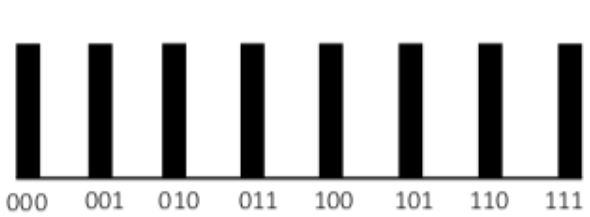
\includegraphics[width=\textwidth]{figures/superposition_carmina}
			\end{figure}
		\end{column}
		\begin{column}{0.1\textwidth}
			$$\longrightarrow$$
		\end{column}
		\begin{column}{0.4\textwidth}  %%<--- here
			
			\begin{figure}[b]
				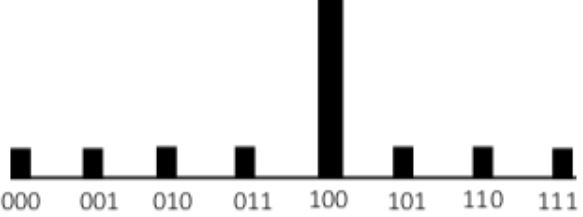
\includegraphics[width=\textwidth]{figures/superposition_carmina_2}
			\end{figure}
				
		\end{column}
	\end{columns}
\end{frame}

\section{Max-Cut}
\begin{frame}{The Max-Cut problem}
\begin{figure}
	\centering
	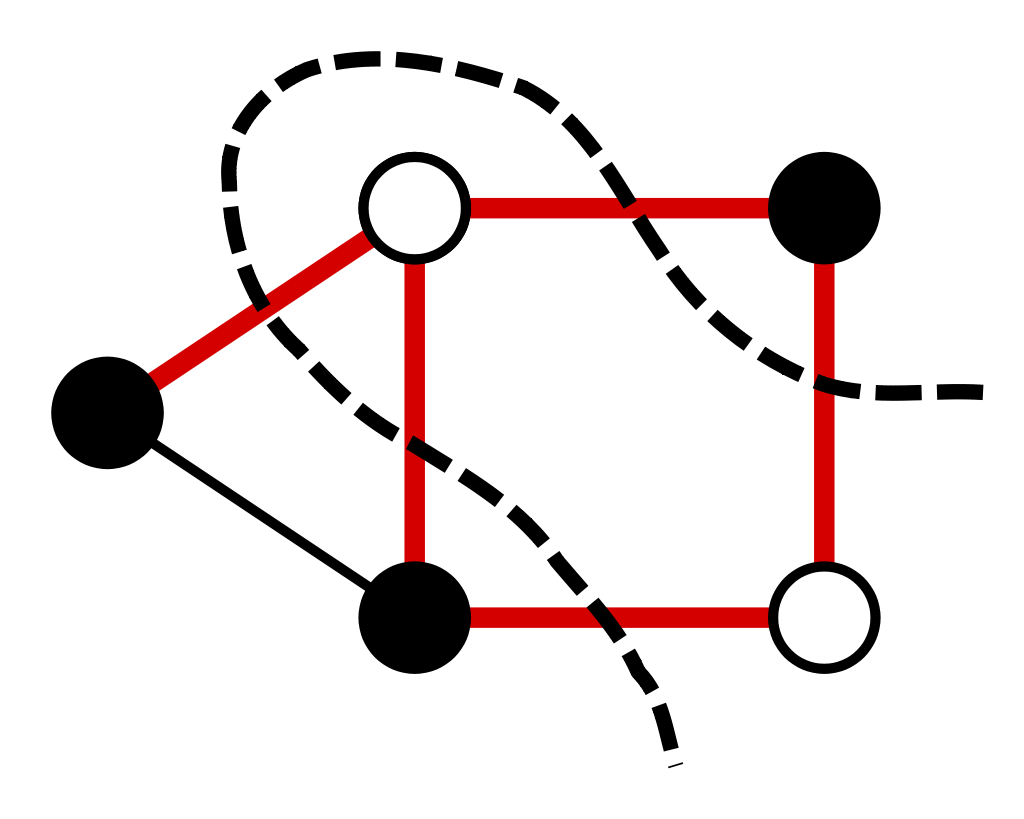
\includegraphics[width=0.8\textwidth]{figures/maxcut}

\end{figure}
\blfootnote{Figure from Wikipedia - Maximum cut}
\end{frame}

\begin{frame}
We would like to find a \textbf{bipartition} that maximizes the following \textbf{cost function}
\begin{equation}
C = \sum_{i\in S, j\in \bar{S}} w_{i,j}
\end{equation}
\pause
Equivalently, we can use a \textbf{binary string} to represent the bipartition
\begin{equation}
C = \sum_{\{i,j\}} \frac{w_{i,j}}{2}(1 - z_i z_j)
\end{equation}

where $\vec{z} \in \{-1,1\}^n$ and $z_i =\begin{cases}
1, & \text{if } \quad i \in S\\
-1, & \text{if } \quad i \in \bar{S}
\end{cases}$
\end{frame}

\section{QAOA}
\subsection{The general algorithm}
\begin{frame}{The Quantum Approximate Optimization Algorithm}
The Quantum Approximate Optimization Algorithm is designed to tackle combinatorial optimization problems. In general, these can be specified with $n$ bits and $m$ clauses. The aim is to satisfy as many clauses as possible
\begin{equation}
C = \sum_{\alpha = 1}^{m} C_{\alpha}
\end{equation}

where $C_{\alpha} =\begin{cases}
1, & \text{if clause $C_{\alpha}$ is satisfied}\\
0, & \text{if clause $C_{\alpha}$ is \emph{not} satisfied}
\end{cases}$
\end{frame}


\begin{frame}{Schematic of the QAOA circuit}
\begin{figure}
	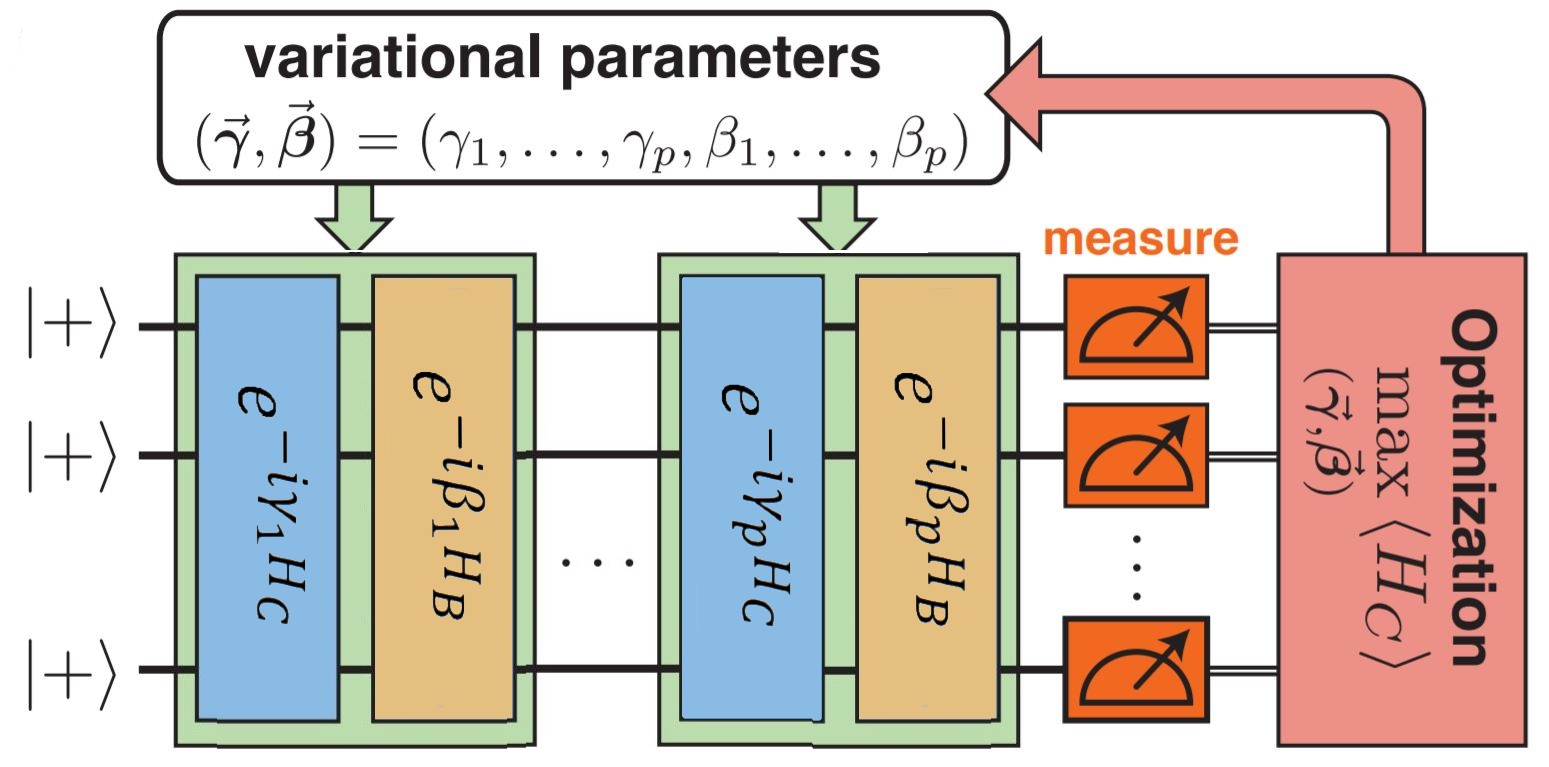
\includegraphics[width=0.9\textwidth]{figures/qaoa_idea_edit_complete}
\end{figure}
\blfootnote{Figure adapted from Zhou et al. Quantum Approximate Optimization Algorithm: Performance, Mechanism, and Implementation on Near-Term Devices (2018)}
\end{frame}

\begin{frame}{The Quantum Part}
\begin{figure}
	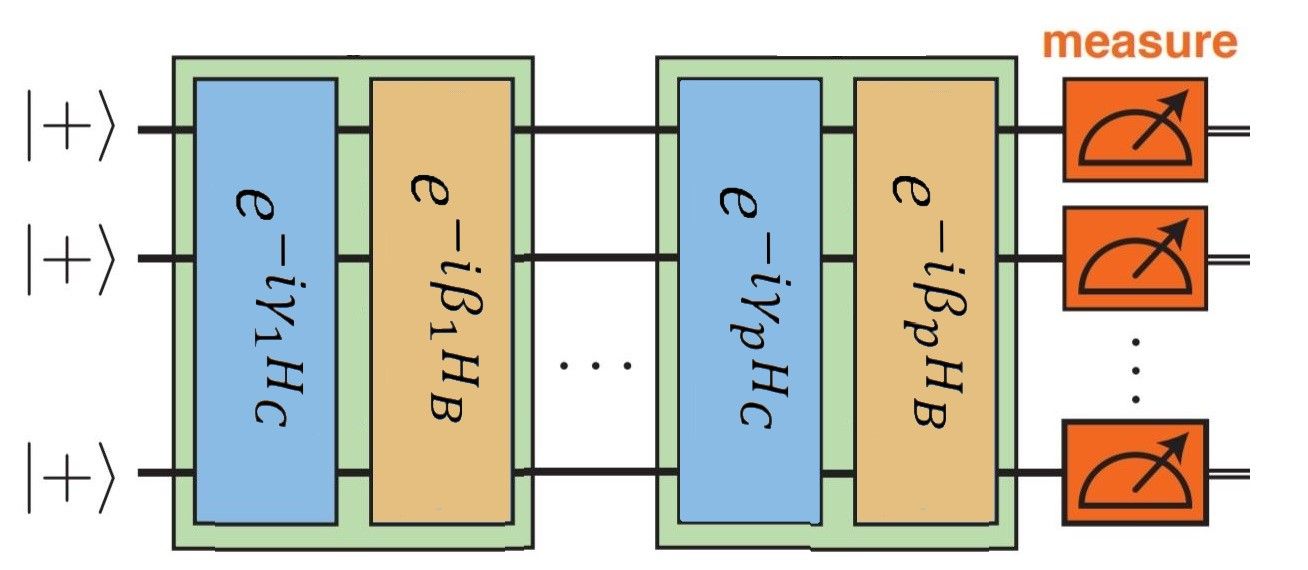
\includegraphics[width=0.9\textwidth]{figures/qaoa_idea_edit}
\end{figure}
\blfootnote{Figure adapted from Zhou et al. Quantum Approximate Optimization Algorithm: Performance, Mechanism, and Implementation on Near-Term Devices (2018)}
\end{frame}

\begin{frame}[t]
	\begin{figure}[t]
		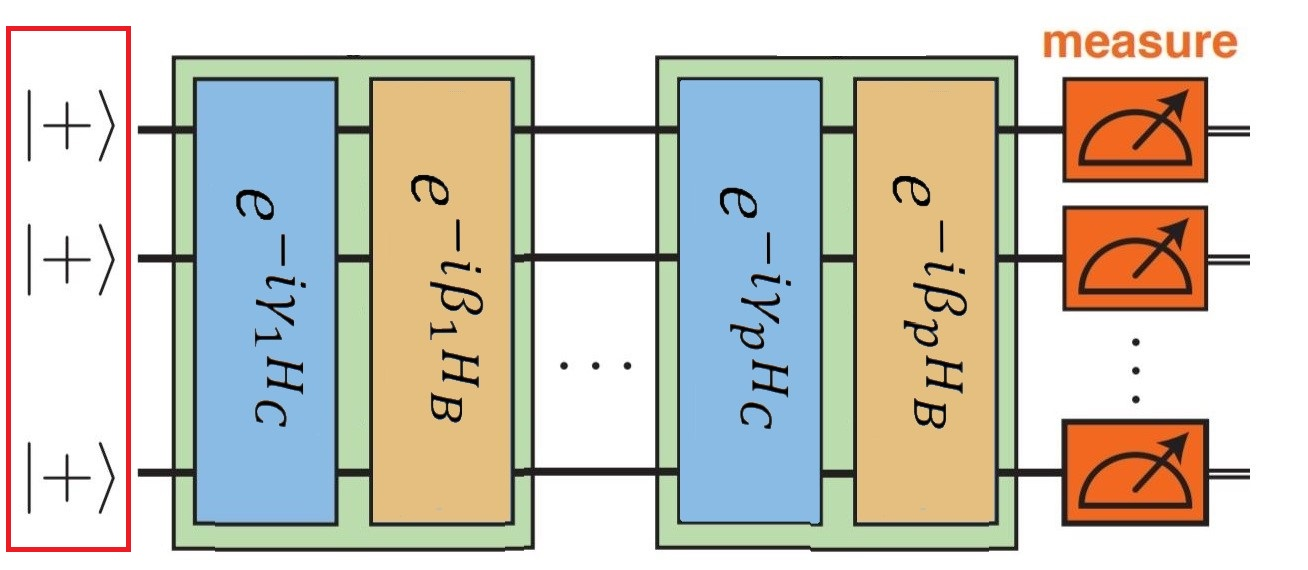
\includegraphics[width=0.6\textwidth]{figures/qaoa_idea_edit_1}
	\end{figure}
	We start from $|+\rangle^{\otimes n}$ which is the \textbf{equal superposition} over all $2^n$ bit strings (or equivalently bipartitions)
	\begin{equation}
	|+\rangle^{\otimes n} = \frac{1}{\sqrt{2^n}}\sum_{\vec{x} \in \{0,1\}^n}|\vec{x}\rangle
	\end{equation}
	
	\pause
	So the amplitude of every bit string is the same
	\begin{figure}
		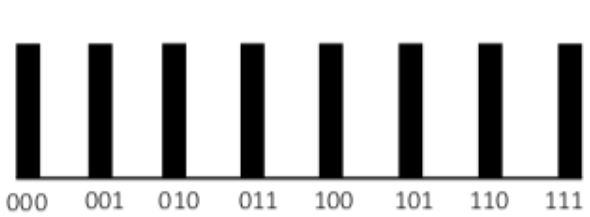
\includegraphics[width=0.4\textwidth]{figures/superposition_carmina}
	\end{figure}
\end{frame}

\begin{frame}[t]
	\begin{figure}[t]
		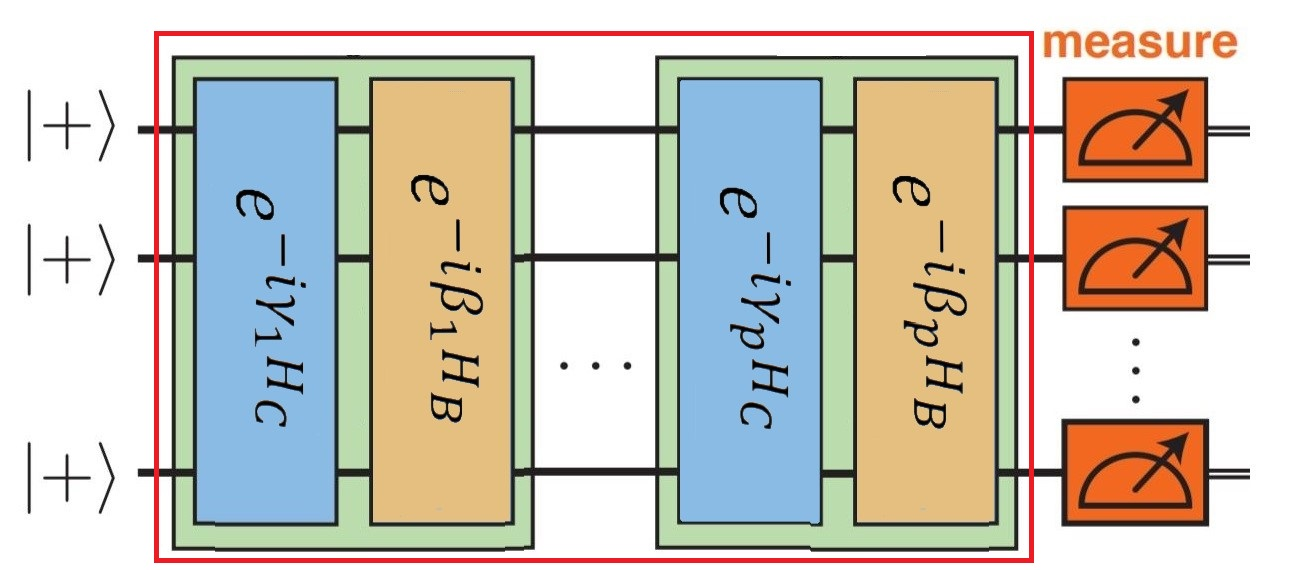
\includegraphics[width=0.6\textwidth]{figures/qaoa_idea_edit_unitaries}
	\end{figure}
\vspace{20px}
Next we alternately apply two gates, the \textbf{cost unitary} and the \textbf{mixer unitary}, derived from two Hamiltonians. \\~\\
We repeat this $p$ times
\end{frame}

\begin{frame}[t]
	\begin{figure}[t]
		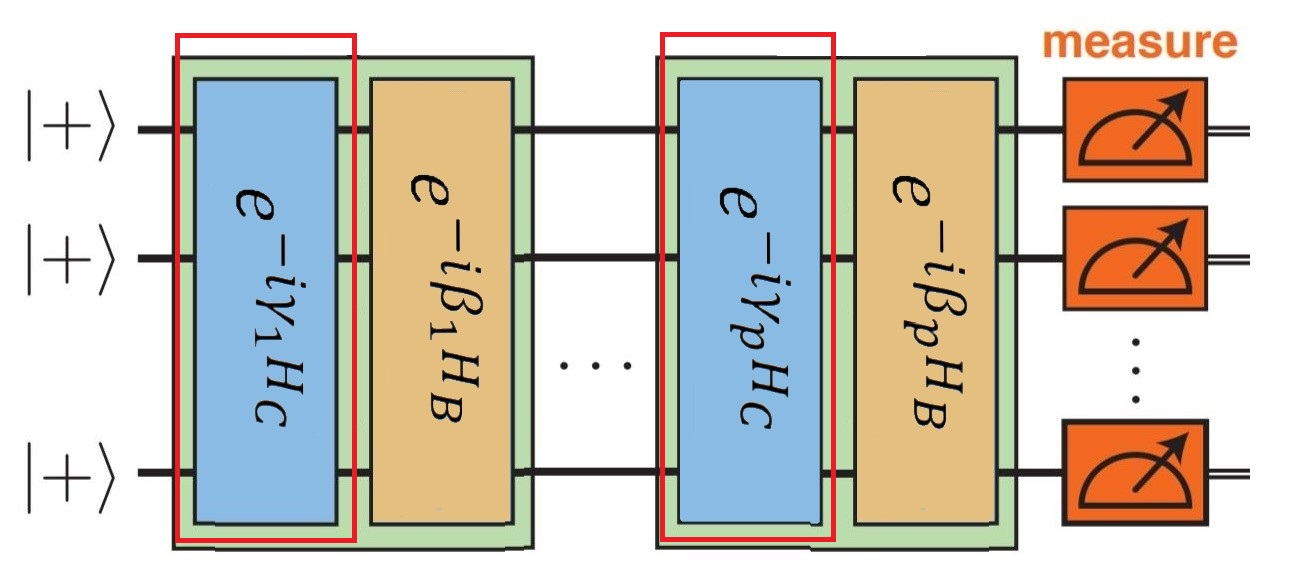
\includegraphics[width=0.6\textwidth]{figures/qaoa_idea_edit_2}
	\end{figure}
\vspace{20px}
	First of the two being the \textbf{cost unitary}. This unitary is derived from the \textbf{cost Hamiltonian} that encodes the objective function $C$
	\begin{equation}
	H_C \equiv \hat{C} = \begin{bmatrix}
	C(0,\dots,0) & &  \\
	& \ddots & \\
	& & C(1,\dots,1)
	\end{bmatrix}
	\end{equation}
\end{frame}

\begin{frame}[t]
\begin{figure}[t]
	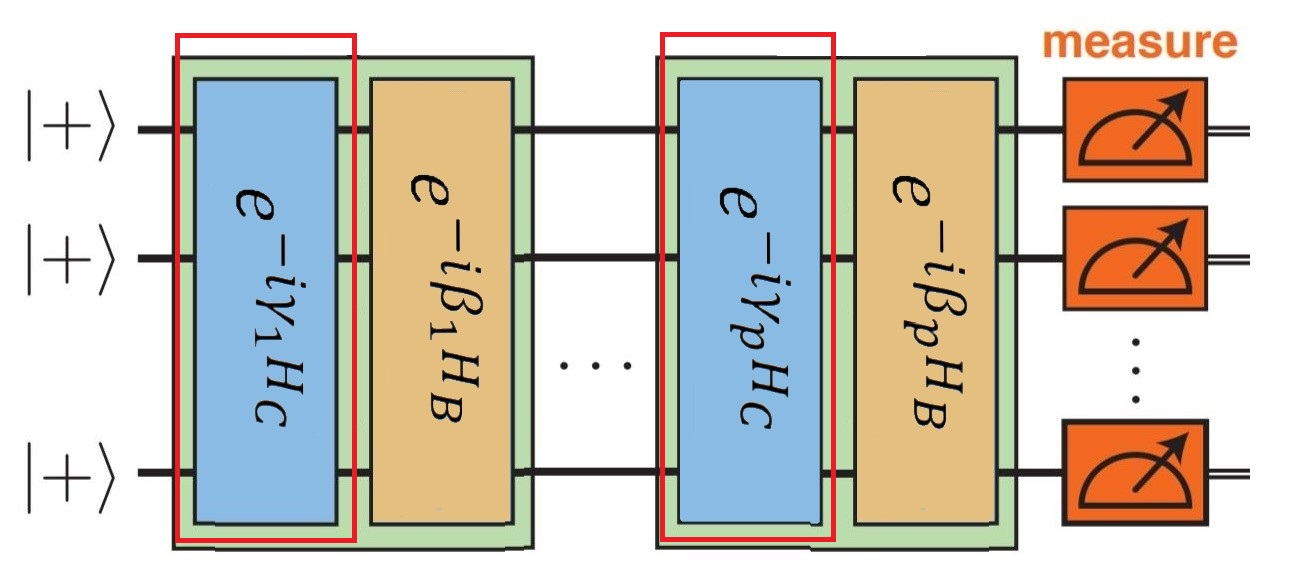
\includegraphics[width=0.6\textwidth]{figures/qaoa_idea_edit_2}
\end{figure}
\vspace{20px}
From the cost Hamiltonian we derive the \textbf{cost unitary}
\begin{equation}
H_C \longrightarrow U(H_C,\gamma)
\end{equation}
with 
\begin{equation}
	U(H_C,\gamma) = e^{-i\gamma H_C}
\end{equation}
for some real parameter $\gamma \in \mathbb{R}$

\end{frame}


\begin{frame}[t]
\begin{figure}[t]
	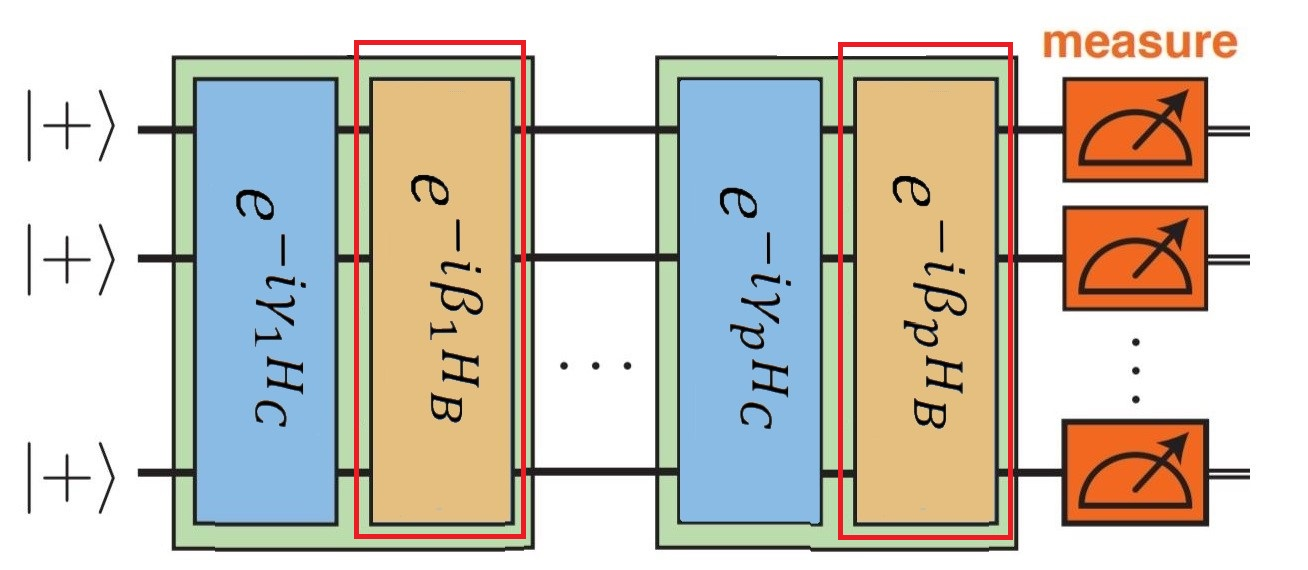
\includegraphics[width=0.6\textwidth]{figures/qaoa_idea_edit_3}
\end{figure}
\vspace{20px}
Secondly, the \textbf{mixer unitary}, derived from the \textbf{mixer Hamiltonian}
\begin{equation}
H_B = \sum_{k = 1}^{n} \sigma_x^{(k)}
\end{equation}

with $\sigma_x^{(k)}$ is the Pauli-$X$ gate applied to the $k$th qubit, which is also called the quantum NOT-gate
\begin{equation}
	\sigma_x = \begin{bmatrix}
	0 & 1 \\
	1 & 0 
	\end{bmatrix}
\end{equation}
\end{frame}

\begin{frame}[t]
\begin{figure}[t]
	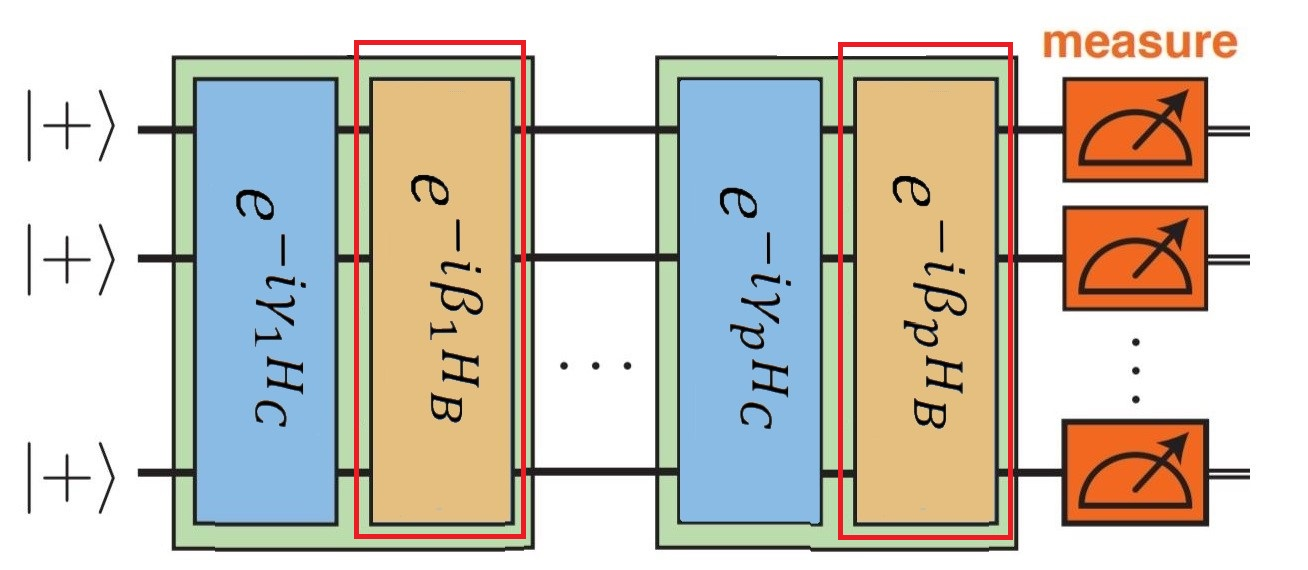
\includegraphics[width=0.6\textwidth]{figures/qaoa_idea_edit_3}
\end{figure}
\vspace{20px}
Analogous to the cost unitary we derive the \textbf{mixer unitary} is derived from the mixer Hamiltonian
\begin{equation}
	H_B \longrightarrow U(H_B,\beta)
\end{equation} 
the mixer unitary is given by
\begin{equation}
	U(H_B,\beta) = e^{-i\beta H_B}
\end{equation}
for some real parameter $\beta \in \mathbb{R}$
\end{frame}

\begin{frame}[t]
\begin{figure}[t]
	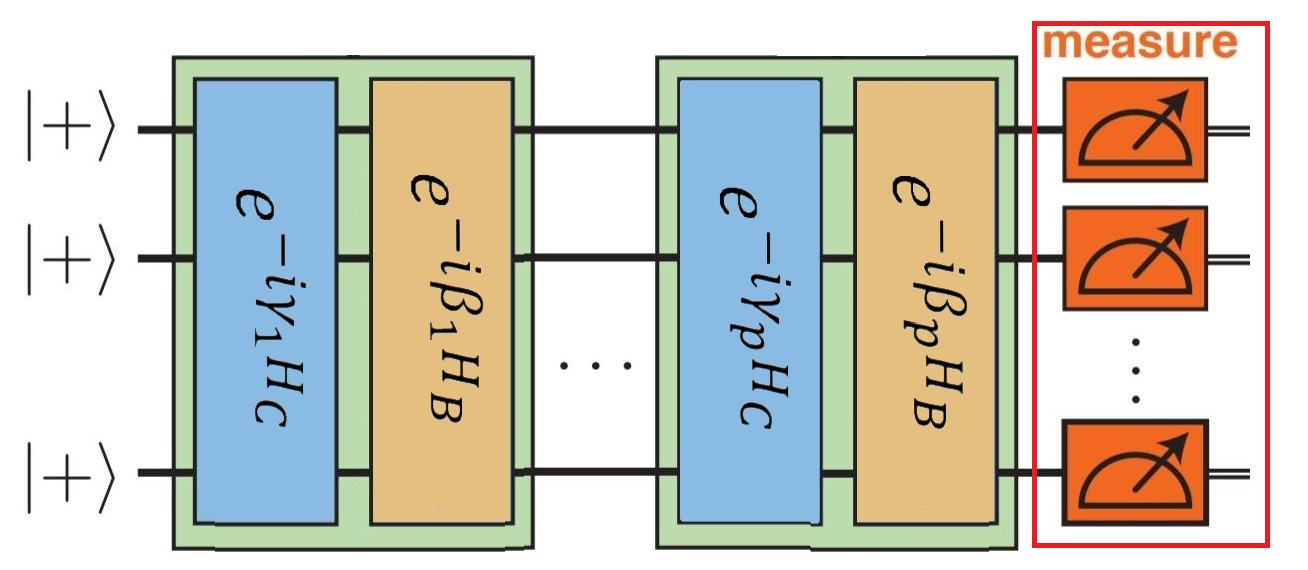
\includegraphics[width=0.6\textwidth]{figures/qaoa_idea_edit_4}
\end{figure}
\vspace{20px}
In the end we prepared the parametrized state
\begin{equation}
	|\gambe\rangle = \underbrace{U(H_B,\beta_p)U(H_C, \gamma_p)\dots \underbrace{U(H_B,\beta_1)U(H_C, \gamma_1)}_{\text{one layer}}}_{p \text{ layers}}|+\rangle^{\otimes n}
\end{equation}
after which we measure the outcome.
\end{frame}


\begin{frame}{The goal: maximize the expectation value}
	Our aim is to prepare a state such that the \textbf{expectation value of the cost Hamiltonian} is maximized
	
	\begin{equation}
		F_p(\gambe) = \langle \gambe | H_C | \gambe \rangle
	\end{equation}
	
	for some sequences of parameters 
	$$\vec{\gamma} = (\gamma_1,\dots,\gamma_p)$$
	$$\vec{\beta} = (\beta_1,\dots,\beta_p)$$
\end{frame}

\subsection{Applying QAOA to Max-Cut}
\begin{frame}{Applying QAOA to Max-Cut}
We \textbf{translate} the objective function into a \textbf{Hamiltonian}
\begin{equation}
C = \sum_{\{i,j\}} w_{i,j}(1 - z_iz_j)
\end{equation}
$$\bigg\downarrow$$
\begin{equation}
H_C = \sum_{\{i,j\}} w_{i,j}\big(I - \sigma_z^{(i)}\sigma_z^{(j)}\big)
\end{equation}

\pause
Using the fact $\sigma_z$ has eigenvalues $1$ and $-1$. Here $\sigma_z^{(i)}$ denotes the Pauli-$Z$ matrix applied to the $i$th qubit.
\begin{equation}
	\sigma_z = \begin{bmatrix}
	1 & 0 \\
	0 & -1
	\end{bmatrix}
\end{equation}
\end{frame}

\begin{frame}{Applying QAOA to Max-Cut}
We can construct the necessary unitaries with local operators
\begin{equation}
	U(H_C, \gamma) = e^{-i\gamma H_C} = \prod_{\{i,j\}\in E} e^{-i\gamma w_{i,j}(1 - \sigma_z^{(i)}\sigma_z^{(j)})}
\end{equation} 
\begin{equation}
	U(H_B,\beta) = e^{-i\beta H_B} = \prod_{k\in V} e^{-i\beta\sigma_x^{(k)}}
\end{equation}
Note that the circuit is dependent on the graph $G = (V,E)$

\vspace{1cm}
Now we are set to construct the circuit for Max-Cut!
\end{frame}

\subsection{Example - the Diamond graph}
\begin{frame}{Example - the Diamond graph}
\begin{figure}
	\centering
	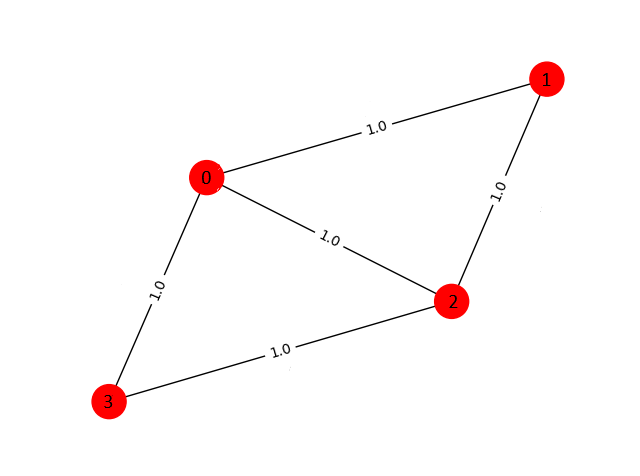
\includegraphics[width=0.9\textwidth]{figures/diamond-graph}
\end{figure}
\end{frame}

\begin{frame}{Example - the circuit}
\begin{figure}
	\centering
	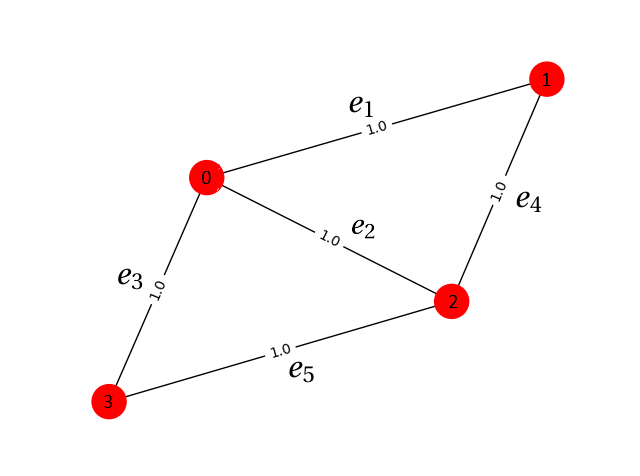
\includegraphics[width=0.55\textwidth]{figures/diamond-graph-edges}
\end{figure}
\begin{figure}
	\centering
	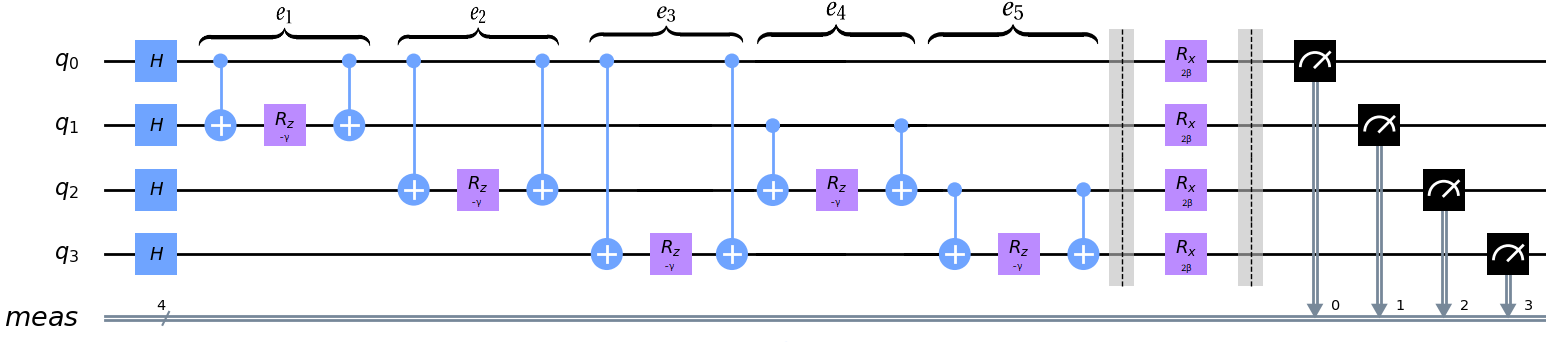
\includegraphics[width=\textwidth]{figures/circuit_diamond_edit2}
\end{figure}
\end{frame}

\begin{frame}{Example - the optimal cut}
\begin{figure}
	\centering
	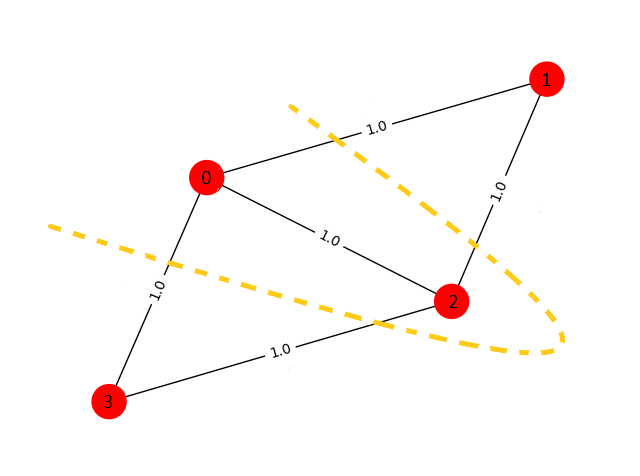
\includegraphics[width=0.9\textwidth]{figures/diamond-graph-cut}
\end{figure}
Note that the optimal cut is $S = \{0,2\}, \bar{S}=\{1,3\}$ or in terms of a binary string $0101$ or $1010$
\end{frame}

\setbeamercovered{transparent}
\begin{frame}{\small{Example - Maximizing the expectation value}}
\captionsetup[subfigure]{labelformat=empty,aboveskip=0pt}
\setlength{\abovecaptionskip}{0pt}
\begin{figure}
	\subfloat[\uncover<1>{\tiny{p=1, $F_1 = 3.24$}}]{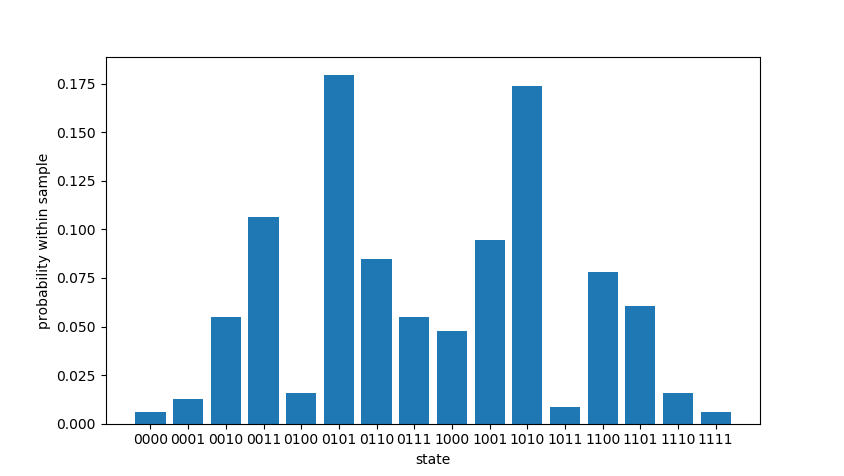
\includegraphics[width=0.475\textwidth]{figures/diamond_p1}}
	\subfloat[]{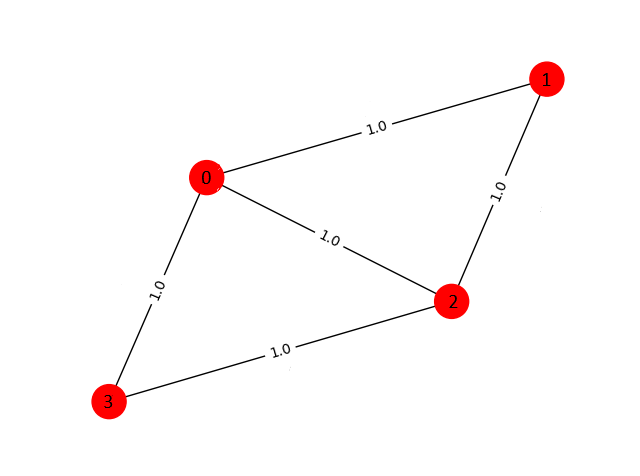
\includegraphics[width=0.475\textwidth]{figures/diamond-graph}}\\
	\subfloat[\uncover<2>{\tiny{p=2, $F_2 = 3.39$}}]{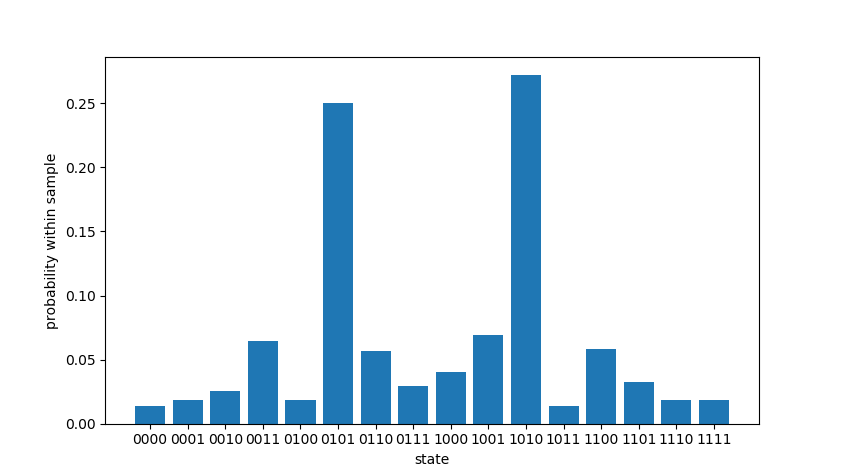
\includegraphics[width=0.475\textwidth]{figures/diamond_p2}}
	\subfloat[\uncover<3>{\tiny{p=3, $F_3 = 3.87$}}]{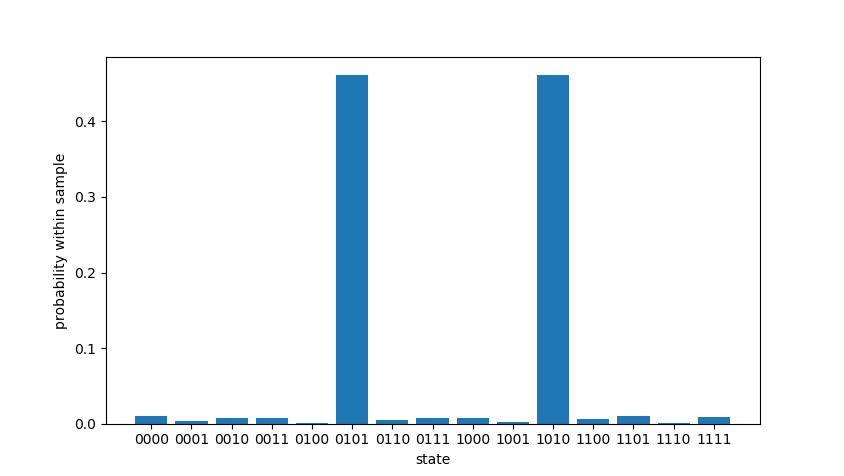
\includegraphics[width=0.475\textwidth]{figures/diamond_p3}}
\end{figure}
\end{frame}

\subsection{How to determine the parameters?}
\begin{frame}{Determining the parameters $\vec{\gamma}, \vec{\beta}$}
\begin{figure}
	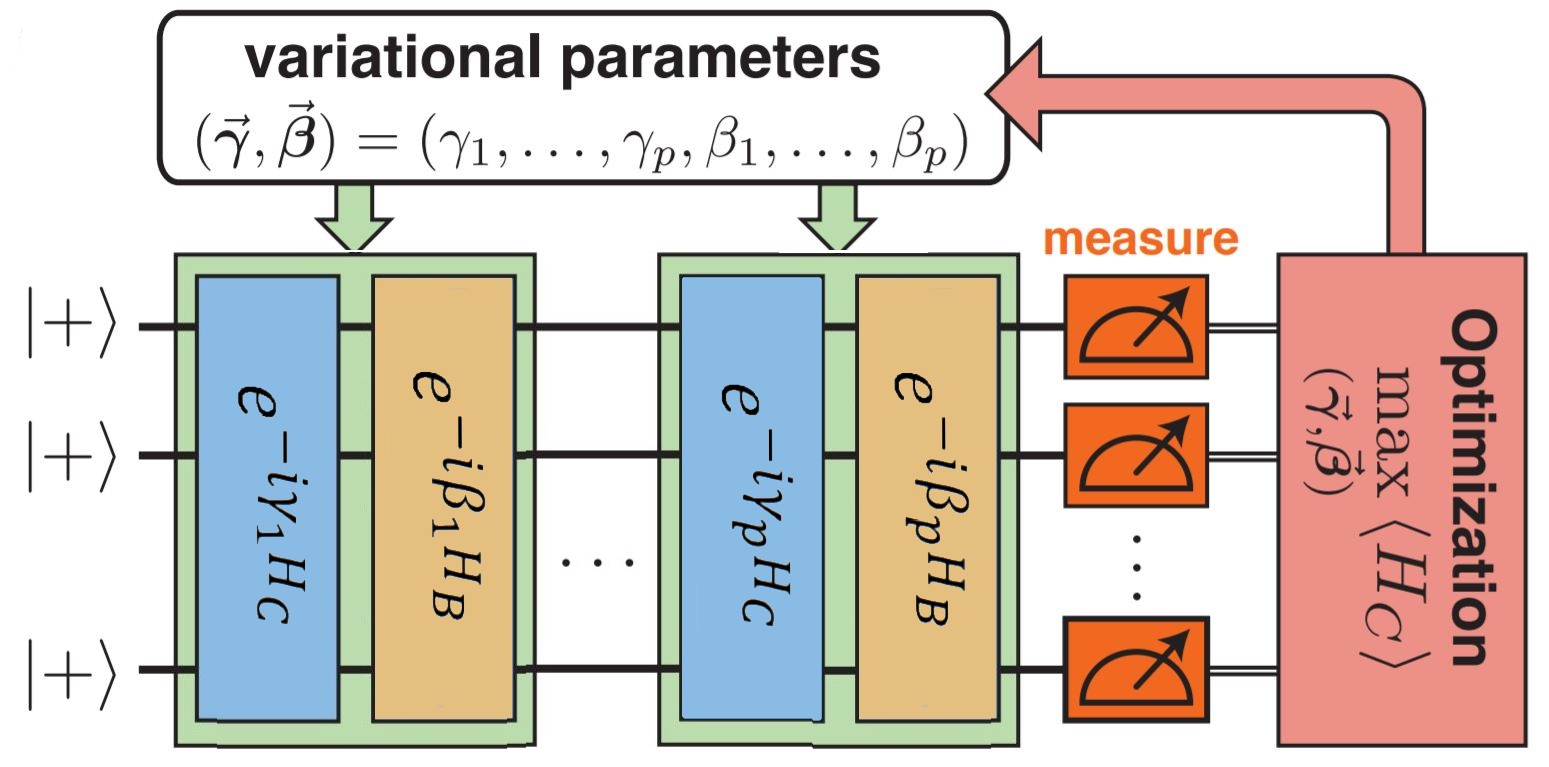
\includegraphics[width=\textwidth]{figures/qaoa_idea_edit_complete}
	\caption{Schematic of the QAOA circuit using VQE optimization.\footnote{Figure adapted from Zhou et al. Quantum Approximate Optimization Algorithm: Performance, Mechanism, and Implementation on Near-Term Devices (2018)}}
\end{figure}
\end{frame}

\subsection{Relation to Quantum Adiabatic Algorithm}
\begin{frame}{Relation to Quantum Adiabatic Algorithm}
\begin{figure}
	\centering
	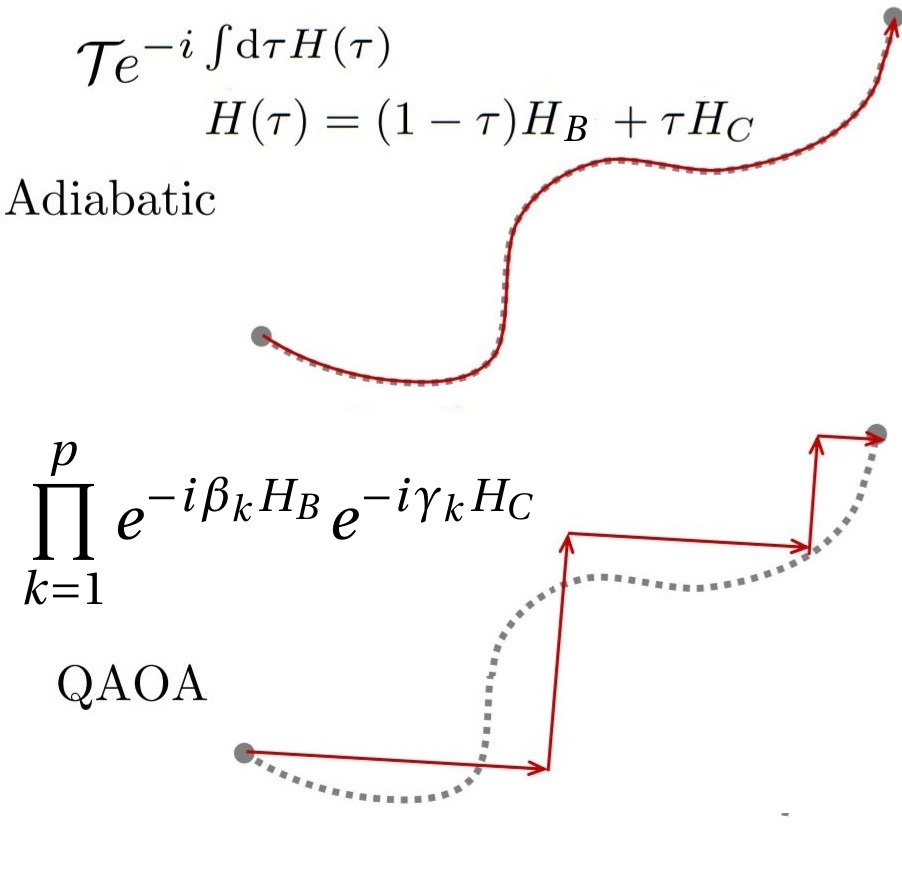
\includegraphics[width=0.6\textwidth]{figures/concept_relation_qaoa_and_qaa_edit}
\end{figure}
\blfootnote{Figure adapted from Verdon et al. A quantum algorithm to train neural networks using low-depth circuits (2017)}
\end{frame}

\begin{frame}{Relation to Quantum Adiabatic Algorithm}
\begin{figure}
	\centering
	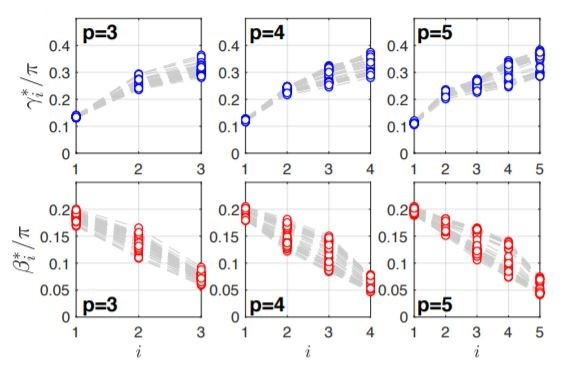
\includegraphics[width=0.8\textwidth]{figures/patterns-u3R}
	\caption{Optimal parameter patterns for unweighted 3-regular graphs with 16 nodes\footnote{Zhou et al. Quantum Approximate Optimization Algorithm: Performance, Mechanism, and Implementation on Near-Term Devices (2018)}}
\end{figure}
\end{frame}

\begin{frame}{Exploiting the relation to QAA - the INTERP method}
\begin{figure}
	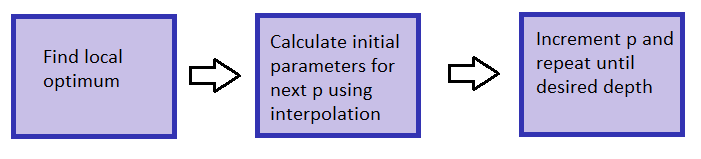
\includegraphics[width=0.8\textwidth]{figures/INTERP}
\end{figure}
\setbeamercovered{invisible}
\captionsetup[subfigure]{labelformat=empty,aboveskip=0pt}
\pause
\begin{figure}
	\subfloat[]{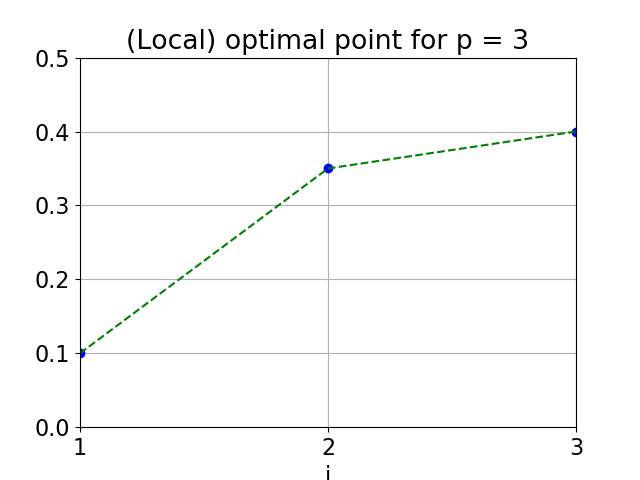
\includegraphics[width=0.45\textwidth]{figures/heuristic_optimal_params.png}}\qquad
	\subfloat[]{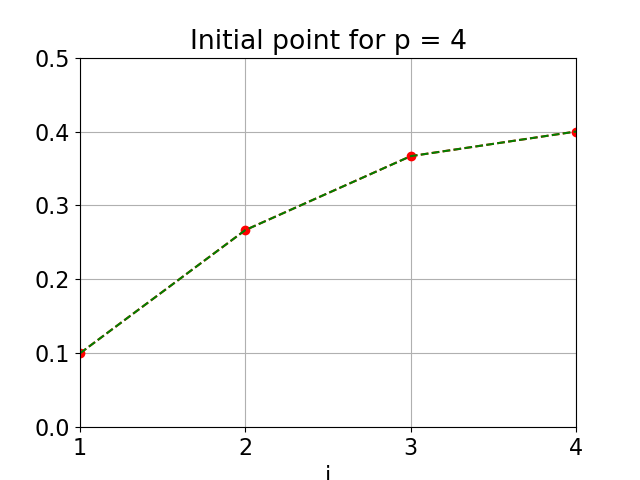
\includegraphics[width=0.45\textwidth]{figures/heuristic_initial_params.png}}
\end{figure}
\end{frame}

\section{My results}
\begin{frame}{My work}
\begin{enumerate}
	\item analysis on \textbf{INTERP method} on different graphs
	\begin{itemize}
		\item cyclic graphs
		\item 3-regular graphs, weighted and unweighted
		\item Erd\H{o}s-R\'enyi graphs
	\end{itemize}
	\item benchmark against \textbf{Goemans-Williamson}, the best known classical approximation algorithm
	\item polynomial time
\end{enumerate}
\end{frame}

\subsection{Found patterns}
\begin{frame}{Found patterns}
\begin{figure}
	\centering
	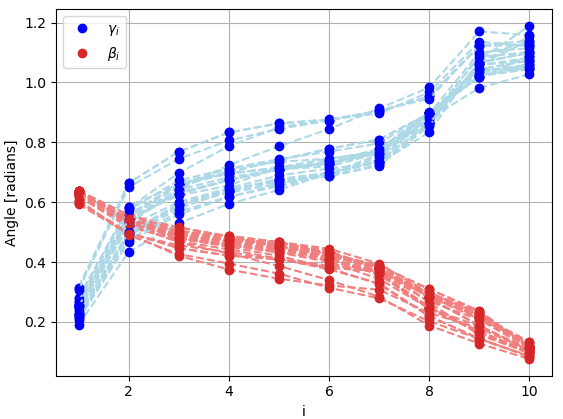
\includegraphics[width=0.9\textwidth]{figures/pattern_3-regular_12-nodal}
\end{figure}
\end{frame}

\subsection{Fractional error}
\begin{frame}{Unweighted 3-regular graphs}
Fractional error $1-r$ decays exponentially with $p$
\captionsetup[figure]{labelformat=empty}
\captionsetup{aboveskip=-3pt}
\begin{figure}
	\centering
	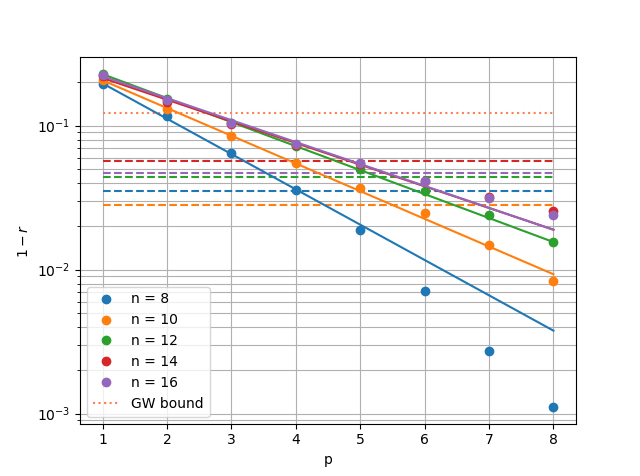
\includegraphics[width=0.8\textwidth]{figures/system-size_unweighted_exp}
	\caption{\tiny{The horizontal lines indicate the average performance of the classical Goemans-Williamson}}
\end{figure}
\end{frame}

\begin{frame}{Weighted 3-regular graphs}
Fractional error $1-r$ decays exponentially with $\sqrt{p}$
\captionsetup[figure]{labelformat=empty}
\captionsetup{aboveskip=-3pt}
\begin{figure}
	\centering
	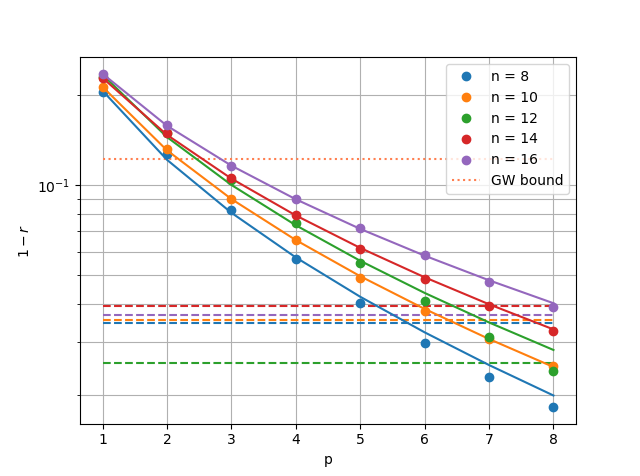
\includegraphics[width=0.8\textwidth]{figures/system-size_sqr}
	\caption{\tiny{The horizontal lines indicate the average performance of the classical Goemans-Williamson}}
\end{figure}

Similar relations were found for the Erd\H{o}s-R\'enyi graphs
\end{frame}

\section{Conclusions and Future Research}
\begin{frame}{Conclusions}
	\begin{itemize}
		\item INTERP beats the classical Goemans-Williamson for relatively low $p \approx 7$ for small graphs
		\pause
		\item The method needs a lot of function evaluations to determine good angles
		\pause
		\item However, this number increases polynomially with $p$ and $n$ so it might offer advantages for large graphs
	\end{itemize}
\end{frame}

\begin{frame}{Thank you!}
	Questions?
\end{frame}

\appendix
\backupbegin
\subsection{Time complexity}
\begin{frame}{Time complexity}
In Zhou et al. (2018) it was claimed the INTERP method is polynomial in $p$, and since the quantum circuit has depth $3m+n$, we find that the complete INTERP method is polynomial in both $n$ and $p$, but is this true in practice?
\begin{figure}
	\centering
	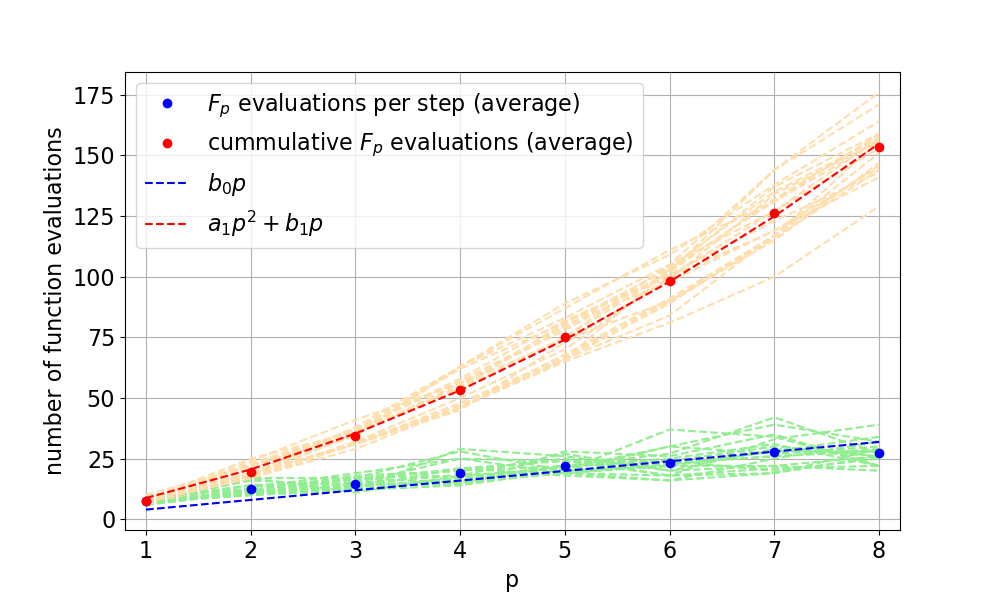
\includegraphics[width=0.9\textwidth]{figures/function_evaluations_16-nodal_unweighted}
\end{figure}
\end{frame}
\backupend

\end{document}
